\chapter{Evaluation}

\section{Cost Benchmark}

This section aims to provide a rough guidance on expected cost for each variant of the smart contract.

Actual costs will vary over time as the Ether-to-USD exchange rate as well as the network gas price will change. It is also dependant of the desired transaction confirmation speed. To avoid this section becoming inaccurate in the future, only the amount of gas consumed is benchmarked. The actual cost can be calculated using the cost model described in chapter 5.

For calculating costs of Ethereum usage, the unit used is gas as it is mostly predictable. This is to make the numbers still usable in the future as gas price and Ether-to-USD conversion rate will experience variance over time.

For variant 1, a benchmark script was created\footnote{The source code can be found under \texttt{v1-gas-benchmark.js}. The benchmark can be executed with \texttt{node index v1-gas-benchmark}.}. The benchmark calculates the cumulative gas spent on contract creation and IP address insertion. Two cases were calculated: For the worst case, each IP address was inserted in a separate transaction. For the best case, reports were bundled into one transaction. The benchmark was executed in both cases for 1 IP address, then 2 IP addresses and so forth up to 20 IP addresses. The resulting costs are displayed in Figure \ref{fig:v1-gas-cost}.

\begin{figure}[H]
\centering
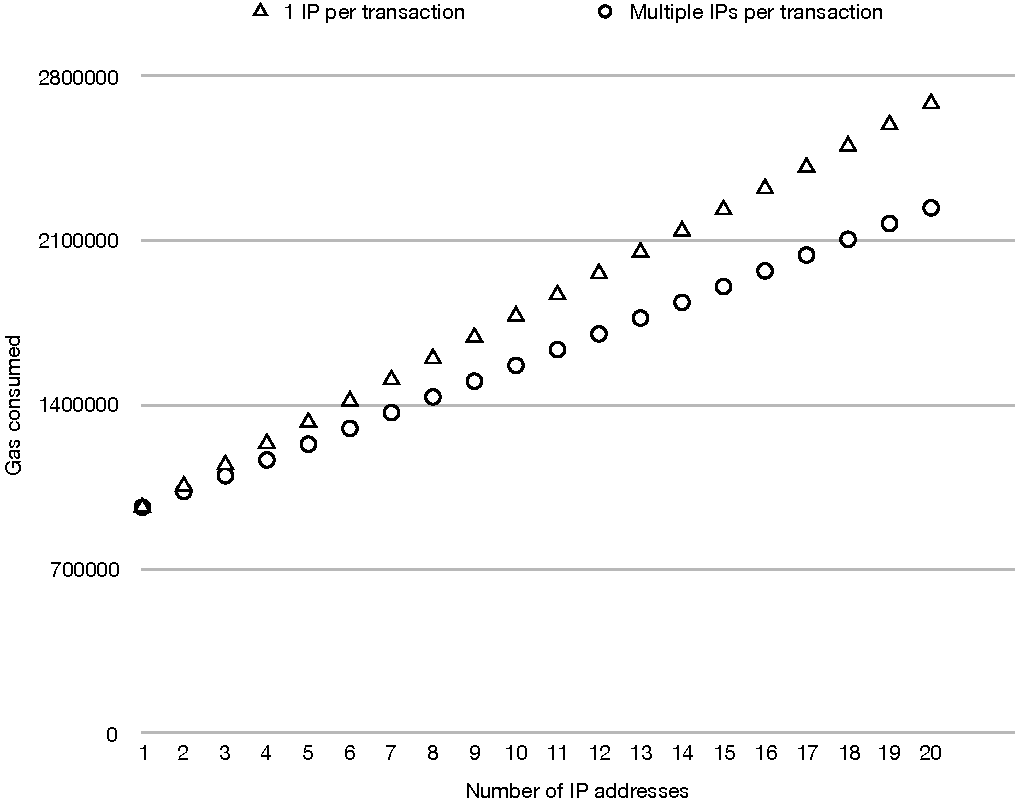
\includegraphics[width=0.7\textwidth]{v1-gas-cost.pdf}
\caption{Gas cost incurred using variant 1}
\label{fig:v1-gas-cost}
\end{figure}

For only a few reports, the major cost is the initial deployment of the contract, costing approximately 858'000 gas. Adding reports costs approximately 150'000 - 200'000 gas each.
It can be observed that bundling reports into one transaction can save 24\% of the gas cost beyond the initial cost (this is however not always practical, as new reports have to be accumulated before they can be bundled, which might make the insertion slower).

Even in the best case, the costs grow linearly ($\mathcal{O}(n)$) as new reports are added. This makes variant 1, as predicted, expensive and unsuitable for big amounts of IP addresses.

\begin{figure}[H]
\centering
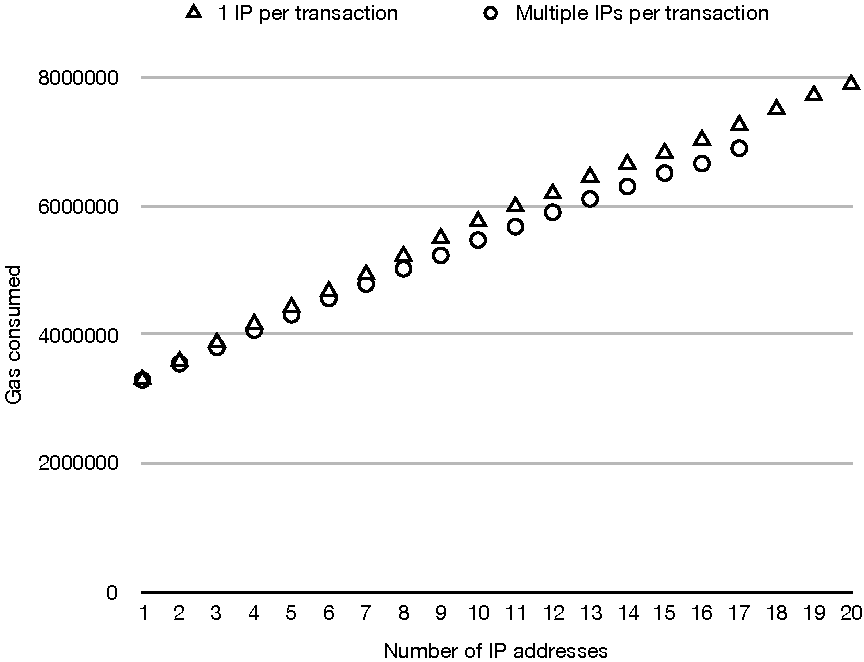
\includegraphics[width=0.7\textwidth]{v3-gas-cost.pdf}
\caption{Gas cost incurred using variant 3}
\label{fig:v3-gas-cost}
\end{figure}

For variant 3 (bloom filter variant), another benchmark script was created\footnote{The source code can be found under \texttt{v3-gas-benchmark.js}. The benchmark can be executed with \texttt{node index v3-gas-benchmark}.}. Like in variant 1, a worst case and a best case scenario was tested, where in the worst case one report gets added at a time, while in the best case, reports could be bundled into one transaction to save gas.

This variant was expected to perform better than variant 1, as less storage is required to store all IP addresses. However, the benchmark does not confirm the expectation. The bloom filter does actually incur more gas costs than storing a full-sized array of IP addresses. 

For adding one report, approximately 290'000 gas is consumed, which is almost three times more than in variant 1 (105'000 gas). There are also no economies of scale, as the cost goes up linearly after the first report. Bundling reports into one transaction does save approximately 40'000 gas per report (13\%), but is less effective than it is for variant 1. Also, it is not possible to add more than 17 reports in one transaction, as the block gas limit is reached.

It becomes clear that Solidity charges more heavily for expensive computation like hashing than it does for storage.
In addition to much higher costs, the bloom filter variant can also give false positives, and metadata like expiration date, whitelist/blacklist etc. has to be stored separately.

If less required storage space does not result in lower prices, then there is no advantage in it at all. The whole blockchain, multiple gigabytes needs to be downloaded to a client anyway \textemdash {} the only reason to optimize for storage is to get cheaper costs.
